
\noindent \textcolor{COLOR2}{RESULTADOS}
\\

\begin{table}[ht]
    \label{tab:resultados}
    \centering
    \begin{tabular}{lc}
        \rowcolor{pagecolor!50!COLOR1}
        \hline
        Modelo & Acurácia (ACC) \\\hline\hline
        LR     & 0.774603       \\\hline
        LDA    & 0.785516       \\\hline
        KNN    & 0.766865       \\\hline
        CART   & 0.681746       \\\hline
        NB     & 0.790278
    \end{tabular}
    \caption{Comparação inicial entre modelos}
\end{table}

A partir de agora, a fim de facilitar a escrita e compreensão, denominar-se-á como:

\begin{itemize}
    \item \textcolor{deepblue}{LDA} - Análise discriminante;
    \item \textcolor{deepblue}{LR} - Regressão Logística;
    \item \textcolor{deepblue}{KNN} - K-ésimo Vizinho mais Próximo;
    \item \textcolor{deepblue}{CART} - Árvore de decisão;
    \item \textcolor{deepblue}{NB} - Naive Bayes;
\end{itemize}

Em primeira mão, analisou-se os modelos com os conjuntos de treinamento para verificar qual deles aparesentaria a \textit{priori} a melhor precisão. Por se tratar de uma comparação entre os modelos, utilizou-se a métrica de acurácia (ACC) para fazer essa avaliação. O Resultado obtido é dado na Tabela \pageref{tab:resultados}.\\

É possível observar pela validação cruzada (Kfold) que o modelo NB apresenta a maior acurácia, com um valor de 0.790278 e o CART o menor com um valor de 0.681746. Verificar-se-á com a execução dos modelos se esse resultado é de fato o encontrado.
\\

\noindent \textcolor{deepblue}{1) LR - REGRESSÃO LOGÍSTICA}
\\
\begin{figure}[!h]
    \centering
    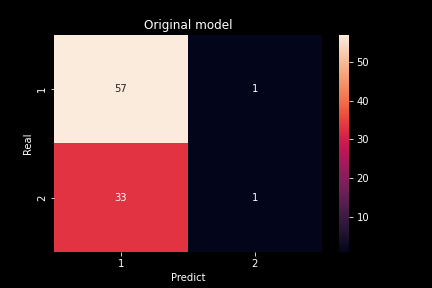
\includegraphics[width=\linewidth, scale=.6]{../../figuras/machine_learning/LR_MC.png}
    \caption{Matriz de confusão da Regressão Logística}
\end{figure}

\begin{table}[!h]
    \centering
    \begin{tabular}{lc}
        \rowcolor{pagecolor!50!COLOR1}
        \hline
        Métrica & Valor   \\\hline\hline
        ACC     & 0.63043 \\\hline
        MCC     & 0.04028 \\\hline
        R       & 0.98275 \\\hline
        P       & 0.63333 \\\hline
        F       & 0.77027
    \end{tabular}
    \caption{LR métricas}
\end{table}

Para o caso da regressão Logística simples, sem nenhum parâmetro de regularização obteve um MCC bastante baixo ($4\%$), muito próximo da aleatoriedade (Tabela 2). Pela matriz de confusão, o modelo indica também que há maior probabilidade de resultados 1, indicando uma sobrevida maior que 5 anos do paciente.\\

Esse modelo obteve uma acurácia muito aquém da validação cruzada feita inicialmente, o que indica uma possibilidade de utilizaçãod e parâmetros de regularização numa tentativa de aumentar esse resultado.
\\

\noindent \textcolor{deepblue}{2) LDA - ANÁLISE DISCRIMINANTE}

\begin{figure}[!h]
    \centering
    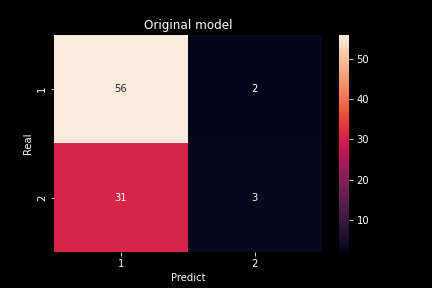
\includegraphics[width=\linewidth, scale=.6]{../../figuras/machine_learning/LDA_MC.png}
    \caption{Matriz de confusão da Análise discriminante}
\end{figure}

\begin{table}[]
    \centering
    \begin{tabular}{lc}
        \rowcolor{pagecolor!50!COLOR1}
        \hline
        Métrica & Valor   \\\hline\hline
        ACC     & 0.64130 \\\hline
        MCC     & 0.11444 \\\hline
        R       & 0.96551 \\\hline
        P       & 0.64367 \\\hline
        F       & 0.77241
    \end{tabular}
    \caption{LDA métricas}
\end{table}

No caso da análise discriminante, quase não houve diferença em relação à regressão Logística. A acurácia se manteve muito parecida, não valendo a pena preteri-la. Há de se observar a situação do Recall (R). O modelo apresenta um valor menor que na regressão logística, sendo o fato prejudicial, já que criar a expectativa de sobrevida maior que 5 anos é uma situação ruim. No caso, falsos negativos são mais prejudiciais que os falso positivos.\\

\noindent \textcolor{deepblue}{3) CART - ÁRVORE DE DECISÃO}


\begin{table}[ht]
    \centering
    \begin{tabular}{lcc}
        \rowcolor{pagecolor!50!COLOR1}
        \hline
        Métrica & Original & Melhorado \\\hline\hline
        ACC     & 0.608696 & 0.630435  \\\hline
        MCC     & 0.119594 & 0.160538  \\\hline
        R       & 0.758621 & 0.793103  \\\hline
        P       & 0.666667 & 0.676471  \\\hline
        F       & 0.709677 & 0.730159
    \end{tabular}
    \caption{CART métricas comparativas}
\end{table}


A árvore de decisão apresentou uma acurácia (ACC) bastante pequena inicialmente. Então, aplicou-se alguns parâmetros de regularização para melhorá-la e ainda assim, não se obteve um resultado satisfatório, sendo ele o menor resultado de todos os modelos ($63\%$).\\

\begin{figure}[H]
    \centering
    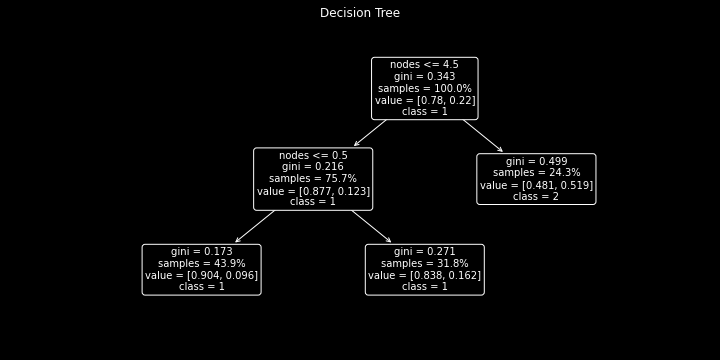
\includegraphics[width=\linewidth, scale=0.5]{../../figuras/machine_learning/cart_tree.png}
    \caption{Árvore de decisão}
\end{figure}

\begin{figure}[H]
    \centering
    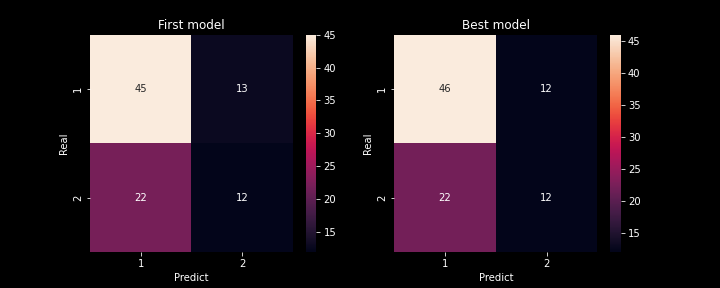
\includegraphics[width=\linewidth, scale=.6]{../../figuras/machine_learning/CART_MC.png}
    \caption{Matriz de confusão comparativa da Árvore de decisão}
\end{figure}

\noindent \textcolor{deepblue}{4) KNN}
\\

Para o KNN, inicialmente obteve-se uma acurácia de $64\%$, o que se encontrou muito parecido com os resultados obtidos anteriormente nas outras análises, apesar de ser um dos maiores ainda assim. Mudou-se então os parâmetros de distância, sendo então testados com as distâncias Euclidiana, de Manhattan e Minkowski e com valores de k variando de 1 a 23. Para uma ditância euclidiana e um k=21, encontrou-se uma acurácia mais elevada correspondente a mais que $70\%$. Tem-se um MCC também mais elevado entre todos os outros modelos, indicando um dado mais próximo do real, além de um R mais elevado. Observa-se qeu o valor de F também se eleva com o aumento de P, o que indica uma maior quantidade de acertos positivos.

\begin{figure}[H]
    \centering
    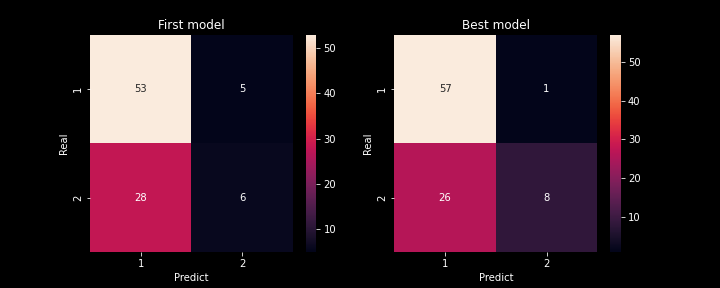
\includegraphics[width=\linewidth, scale=.6]{../../figuras/machine_learning/KNN_MC.png}
    \caption{Matriz de confusão comparativa do modelo KNN}
\end{figure}

\begin{table}[ht]
    \centering
    \begin{tabular}{lcc}
        \rowcolor{pagecolor!50!COLOR1}
        \hline
        Métrica & Original & Melhorado \\\hline\hline
        ACC     & 0.641304 & 0.706522  \\\hline
        MCC     & 0.134285 & 0.354287  \\\hline
        R       & 0.913793 & 0.982759  \\\hline
        P       & 0.654321 & 0.686747  \\\hline
        F       & 0.762590 & 0.808511
    \end{tabular}
    \caption{KNN métricas originais e ajustadas}
\end{table}

\noindent \textcolor{deepblue}{5) NB - NAIVE BAYES}
\\

Inicialmente, o modelo NB apresentou o maior valor de precisão com a avaliação cruzada do conjunto de treinamento. Todavia, após a análise com o conjunto de testes, verificou-se que os resultados encontrados não apresentam nenhuma tendência de melhora com ajuste de parâmetros e também com todos os valores inferiores ao KNN ajustado, por exemplo. A matriz de confusão continua a mostrar uma prevalecência de valores 1 em ambos os casos.

\begin{table}[ht]
    \centering
    \begin{tabular}{lcc}
        \rowcolor{pagecolor!50!COLOR1}
        \hline
        Métrica & Original & Melhorado \\\hline\hline
        ACC     & 0.652174 & 0.652174  \\\hline
        MCC     & 0.162579 & 0.162579  \\\hline
        R       & 0.965517 & 0.965517  \\\hline
        P       & 0.651163 & 0.651163  \\\hline
        F       & 0.777778 & 0.777778
    \end{tabular}
    \caption{NB métricas originais e ajustadas}
\end{table}

\begin{figure}[H]
    \centering
    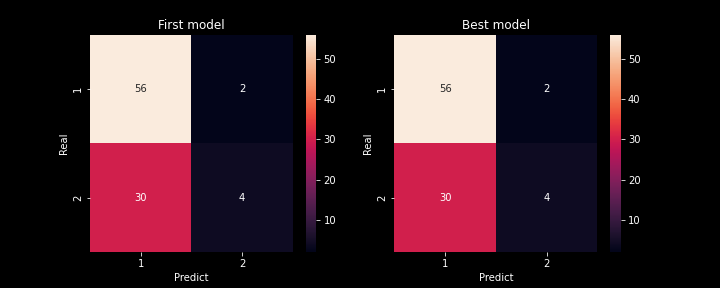
\includegraphics[width=\linewidth, scale=.6]{../../figuras/machine_learning/NB_MC.png}
    \caption{Matriz de confusão comparativa do modelo Naive Bayes}
\end{figure}


\noindent \textcolor{COLOR2}{CONCLUSÃO}
\\